\newpage
\section{実験}
  本研究ではHuda Fitriyaniらの実験\cite{puzzle}に倣い,
  1日10回のパズル活動を実物で2週間,
  VR上で2週間の2回に分けて,計4週間行う.
  \\\indent
  被験者は小学校低学年20名で,10名ずつの2つのグループに分ける.
  グループAは1回目にVRで実験を行い,
  2回目は実物で行う.
  グループBは1回目に実物で行い,
  2回目はVRで行う.
  実験の流れを図\ref{flow}に示す.
  %======================================================================================
  \begin{figure}[h]
    \begin{center}
      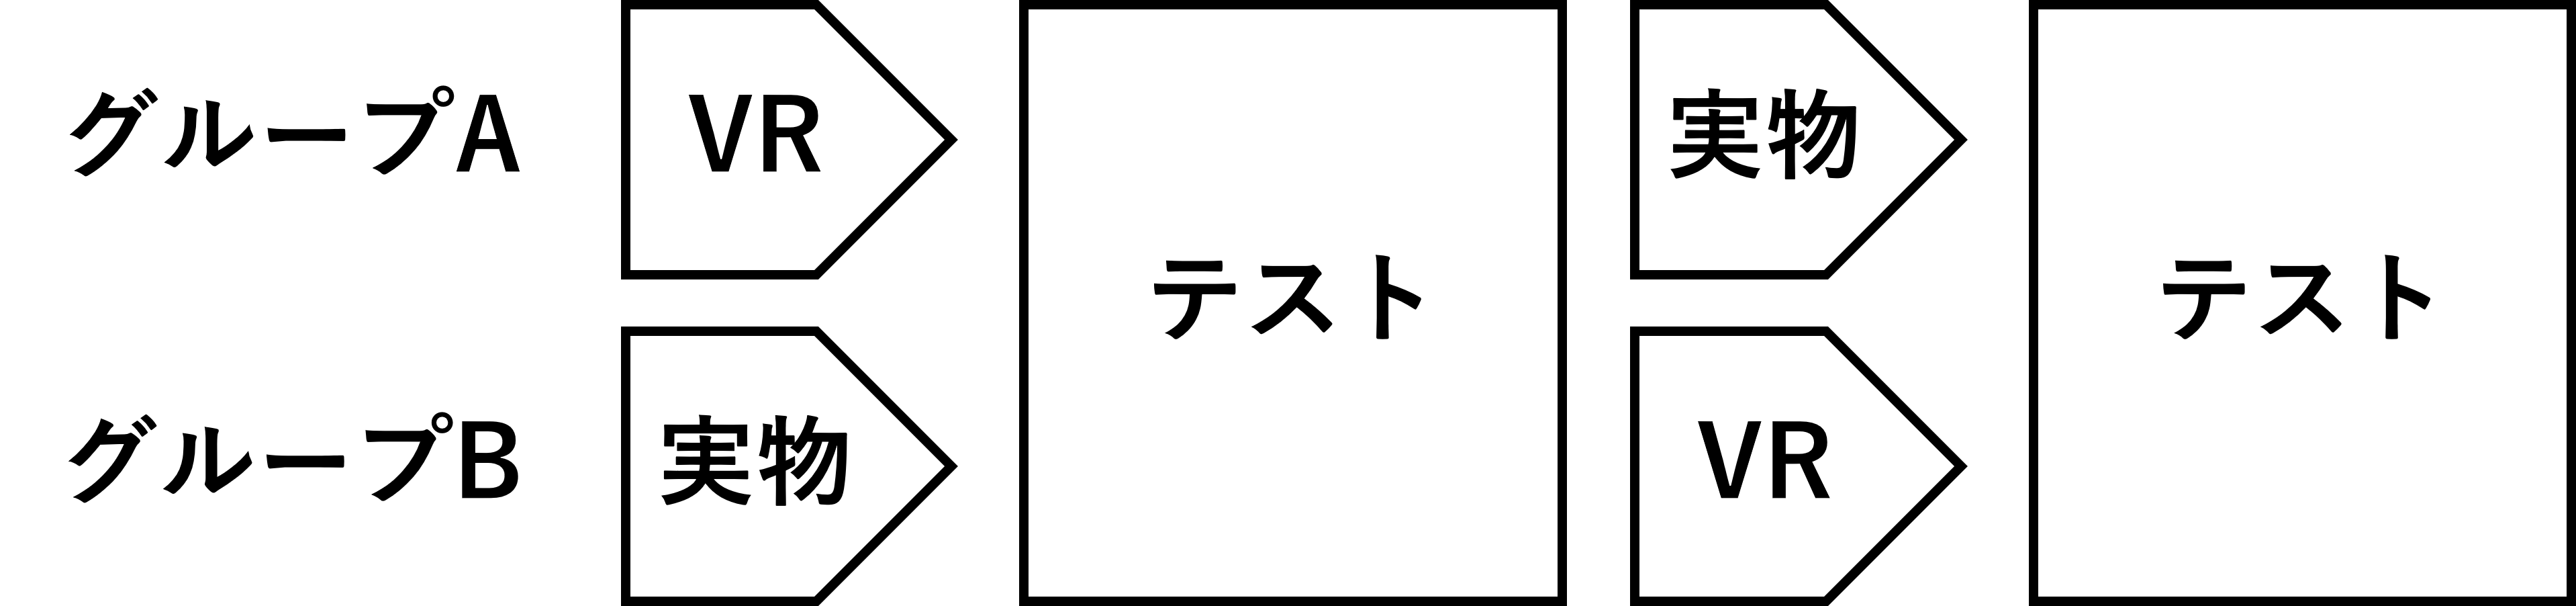
\includegraphics[width=80mm]{./images/experiment.png}
      \caption{実験の流れ}\label{flow}
    \end{center}
  \end{figure}
  %======================================================================================
